\documentclass{ctexart}

\usepackage{amsmath}
\usepackage{amssymb}
\usepackage{subfigure}
\usepackage[graphicx]{realboxes}
\counterwithin{figure}{section}

\begin{document}

\section{复数的代数表示}
\flushleft{一个复数A可以用下述几种形式来表示,}
\begin{align*}
A &= a + jb \quad &\text{代数式} \\
  &= r(\cos\psi + j\sin\psi) \quad &\text{三角式} \\
  &= re^{j\psi} \quad &\text{指数式} \\
  &= r\angle\psi \quad &\text{极坐标式}
\end{align*}
\flushleft{其中$r = \sqrt{a^2 + b^2},\tan\psi = \frac{b}{a},\psi = \arctan{\frac{b}{a}},e^{j\psi} = \cos\psi + j\sin\psi$}
\flushleft{复数的加减运算常用代数形式,而乘除运算则常用指数式和极坐标式}

\section{正弦交流电路的视在功率}
\flushleft{负载的视在功率:}
\begin{gather*}
S = UI
\end{gather*}
\flushleft{平均功率、无功功率和视在功率间存在着一定的联系:}
\begin{gather*}
S = \sqrt{P^2 + Q^2}
\end{gather*}

\newpage

\section{相量的四则运算}
\flushleft{令:$A = a_1 + jb_1, B = a_2 + jb_2$}
\flushleft{加减运算:}
\begin{gather*}
A \pm B = (a_1 \pm a_2) + j(b_1 \pm b_2)
\end{gather*}
\flushleft{乘除运算:}
\begin{gather*}
AB = r_{a}e^{j \psi_a} \cdot r_{b}e^{j \psi_b} = r_{a}r_{b}e^{j(\psi_a + \psi_b)} \\
AB = r_a\angle\psi_a \cdot r_b\angle\psi_b = r_{a}r_{b}\angle(\psi_a + \psi_b) \\
\frac{A}{B} = \frac{a_1 + jb_1}{a_2 + jb_2} = \frac{(a_1 + jb_1)(a_2 - jb_2)}{(a_2 + jb_2)(a_2 - jb_2)} = \frac{a_{1}a_{2} + b_{1}b_{2}}{a^2_2 + b^2_2} + j\frac{a_{2}b_{1} - a_{1}b_{2}}{a^2_2 + b^2_2} \\
\frac{A}{B} = \frac{r_{a}e^{j\psi_a}}{r_{b}e^{j\psi_b}} = \frac{r_a}{r_b}e^{j(\psi_a - \psi_b)} \\
\frac{A}{B} = \frac{r_a\angle\psi_a}{r_b\angle\psi_b} = \frac{r_a}{r_b}\angle(\psi_a - \psi_b)
\end{gather*}

\section{阻抗的并联}
\begin{gather*}
\frac{1}{Z} = \sum_{k=1}^n \frac{1}{Z_k}
\end{gather*}

\section{周期和频率}
\flushleft{周期T:正弦量变化一周所需要的时间}
\flushleft{频率$f = \frac{1}{T}$}
\flushleft{角频率$\omega = \frac{2\pi}{T} = 2\pi f$}

\newpage

\section{正弦函数的相位差}
\flushleft{某元件端电压 u 和流过的电流 i 频率相同,}
\begin{gather*}
u = U_m\sin(\omega t + \psi_u) \\
i = I_m\sin(\omega t + \psi_i) \\
\psi = (\omega t + \psi_u) - (\omega t + \psi_i) = \psi_u - \psi_i
\end{gather*}
\flushleft{$\psi = \psi_u - \psi_i > 0$说明u总比i先经过最大值,u超前于i}
\flushleft{$\psi = \psi_u - \psi_i = 0$说明u和i的初相相同,或者说u和i同相}
\flushleft{$\psi = \psi_u - \psi_i = 180^\circ$说明u和i相位相反,或者说u和i反相}

\section{基尔霍夫定律的相量形式}
\flushleft{KCL 的相量形式:}
\begin{gather*}
\sum_{k=1}^n \dot{I}_k = 0
\end{gather*}
\flushleft{KVL 的相量形式:}
\begin{gather*}
\sum_{k=1}^n \dot{U}_k = 0
\end{gather*}

\section{相量表示法}
\flushleft{例如正弦电压,则表示它的相量为:}
\begin{gather*}
\dot{U}_m = U_m(\cos\psi + j\sin\psi) = U_{m}e^{j\psi} = U_m\angle\psi \\
\dot{U} = U(\cos\psi + j\sin\psi) = Ue^{j\psi} = U\angle\psi
\end{gather*}
\flushleft{注意:相量是正弦量的表示,但不相等,即$u \ne \dot{U} \ne U$}

\newpage

\section{电容中的功率}
\flushleft{设$i = I_m\sin(\omega t + \frac{\pi}{2}), u = U_m\sin\omega t$}
\flushleft{则电容元件的瞬时功率为:}
\begin{gather*}
p = ui = U_m\sin\omega t \cdot I_m\sin(\omega t + \frac{\pi}{2}) = U_{m}I_{m}\sin\omega t\cos\omega t = UI\sin2\omega t
\end{gather*}
\flushleft{则电容元件的平均功率为:}
\begin{gather*}
P = P_C = \frac{1}{T}\int_{0}^{T}pdt = UI\sin2\omega tdt = 0
\end{gather*}

\section{电感中的功率}
\flushleft{设$i = I_m\sin\omega t, u = U_m\sin(\omega t + \frac{\pi}{2})$}
\flushleft{则电感元件的瞬时功率为:}
\begin{gather*}
p = ui = U_m\sin(\omega t + \frac{\pi}{2}) \cdot I_m\sin\omega t = U_{m}I_{m}\cos\omega t\sin\omega t = UI\sin2\omega t
\end{gather*}
\flushleft{则电感元件的平均功率为:}
\begin{gather*}
P = P_L = \frac{1}{T}\int_{0}^{T}pdt = UI\sin2\omega tdt = 0
\end{gather*}

\newpage

\section{正弦交流电路的功率}
\flushleft{设交流负载的端电压u和端电流i之间存在相位差,因此负载的端电压u和端电流i之间的关系可表示为:}
\begin{align*}
i &= I_m\sin\omega t \\
u &= U_m\sin(\omega t + \phi)
\end{align*}
\flushleft{负载取用的瞬时功率为:}
\begin{align*}
p &= ui = U_{m}I_{m}\sin\omega t\sin(\omega t + \phi) \\
  &= 2UI\sin\omega t\sin(\omega t + \phi) \\
  &= UI\cos\phi - UI\cos(2\omega t + \phi)
\end{align*}
\flushleft{负载的平均功率(即有功功率)为:}
\begin{gather*}
P = \frac{1}{T}\int_{0}^{T}pdt = \frac{1}{T}\int_{0}^{T}[UI\cos\phi - UI\cos(2\omega t + \phi)]dt = UI\cos\phi
\end{gather*}
\flushleft{负载的无功功率为:}
\begin{gather*}
Q = UI\sin\phi
\end{gather*}

\section{阻抗的串联}
\begin{gather*}
Z = \sum_{k=1}^n Z_k = \sum_{k=1}^n R_k + j\sum_{k=1}^n X_k = \left\vert Z \right\vert \angle\phi \\
\left\vert Z \right\vert = \sqrt{(\sum R_k)^2 + (\sum X_k)^2},\quad \phi = \arctan\frac{\sum X_k}{\sum R_k}
\end{gather*}
\flushleft{串联总阻抗的电阻值等于各部分电阻之和,总电抗等于各部分电抗的代数和,注意其中感抗取正号,容抗取负号。}
\begin{gather*}
\dot{U}_k = \dot{I}Z_k = \frac{\dot{U}}{Z}Z_k
\end{gather*}

\section{电容中电压和电流的关系}
\flushleft{设$u_C = U_m\sin\omega t$}
\begin{align*}
i_C &= C\frac{du}{dt} = C \cdot \frac{d(U_m\sin\omega t)}{dt} \\
    &= \omega C \cdot U_m\cos\omega t \\
    &= \omega C \cdot U_m\sin(\omega t + 90^\circ) \\
    &= I_m\sin(\omega t + 90^\circ)
\end{align*}
\flushleft{$u_C$和$i_C$是同频率的正弦量并且在相位上$u_C$滞后于电流$i_C$$90^\circ$}

\section{电感中电压和电流的关系}
\flushleft{设$i_L = I_m\sin\omega t$}
\begin{align*}
u_L &= L\frac{di_L}{dt} = L\frac{d(I_m\sin\omega t)}{dt} \\
    &= \omega L I_m\cos\omega t \\
    &= \omega L I_m\sin(\omega t + 90^\circ) \\
    &= U_m\sin(\omega t + 90^\circ)
\end{align*}
\flushleft{$u_L$和$i_L$是同频率的正弦量并且在相位上$u_L$超前于电流$i_L$$90^\circ$}

\section{微积分第二基本定理}
\flushleft{如果函数f(x)在区间[a, b]上连续,并且存在原函数F(x),则}
\begin{gather*}
\int_{a}^{b} f(x)dx = F(b) - F(a)
\end{gather*}

\newpage

\section{RLC串联交流电路中的总阻抗}
\flushleft{Z为R、L、C元件串联后的总阻抗:}
\begin{gather*}
Z = R + j(\omega L - \frac{1}{\omega C}) = R + jX = \sqrt{R^2 + X^2}\angle\arctan\frac{X}{R} = \left\vert Z \right\vert \angle\phi
\end{gather*}
\flushleft{其中:}
\begin{gather*}
\left\vert Z \right\vert = \sqrt{R^2 + X^2} = \sqrt{R^2 + (X_L - X_C)^2} \\
\phi = \arctan\frac{X}{R} = \arctan\frac{X_L - X_C}{R}
\end{gather*}

\section{RLC串联交流电路中的电压}
\flushleft{瞬时值表达式:}
\begin{align*}
u &= u_R + u_L + u_C \\
  &= RI_m\sin\omega t + \omega LI_m\sin(\omega t + 90^\circ) + \frac{1}{\omega C}I_m\sin(\omega t - 90^\circ)
\end{align*}
\flushleft{相量表达式:}
\begin{align*}
\dot{U} &= \dot{U}_R + \dot{U}_L + \dot{U}_C \\
        &= R\dot{I} + j\omega L\dot{I} - j\frac{1}{\omega C}\dot{I} = [R + j(\omega L - \frac{1}{\omega C})]\dot{I} \\
        &= (R + jX)\dot{I} = Z\dot{I}
\end{align*}

\section{N沟道增强型MOS管工作在放大区时的漏极电流}
\flushleft{在放大区(恒流区)内,N沟道增强型MOS管的$I_{D}$可近似地表示为:}
\begin{gather*}
I_{D} = I_{DO}(\frac{U_{GS}}{U_{GS(th)}} - 1)^2
\end{gather*}
\flushleft{上式中,$I_{DO}$是$U_{GS}=2U_{GS(th)}$时$I_{D}$的值}

\section{放大倍数}
\flushleft{电压放大倍数:$\dot{A_u} = \frac{\dot{U_o}}{\dot{U_i}}$}
\flushleft{电流放大倍数:$\dot{A_i} = \frac{\dot{I_o}}{\dot{I_i}}$}
\flushleft{功率放大倍数:$A_p = \frac{p_o}{p_i}$}

\section{固定偏置共发射极放大电路中电压电流关系}
\flushleft{当$u_i = 0$时,放大电路所处的状态称为直流状态或静止工作状态,简称静态。此时三极管的输入特性和输出特性曲线上有一个确定的静态工作点,称之为Q点,它对应有一定的$I_{BQ}$、$U_{BEQ}$、$I_{CQ}$和$U_{CEQ}$。}
\flushleft{当放大电路加入输入交流信号,如十几到几十毫伏,这时电路为动态工作状态,发射结电压瞬时值为:}
\begin{gather*}
u_{BE} = U_{BEQ} + u_{be} = U_{BEQ} + u_i
\end{gather*}
\flushleft{基极电流瞬时值为:}
\begin{gather*}
i_B = I_{BQ} + i_b
\end{gather*}
\flushleft{三极管工作在放大区,具有集电极电流受基极电流控制的情况,因此:}
\begin{gather*}
i_C = \beta i_B = \beta(I_{BQ} + i_b) = \beta I_{BQ} + \beta i_b = I_{CQ} + i_c
\end{gather*}
\flushleft{在输出回路中,由KVL定律可写出电压方程:}
\begin{align*}
u_{CE} &= V_{CC} - i_{C}R_{C} = V_{CC} - (I_{CQ} + i_c)R_C \\
       &= V_{CC} - I_{CQ}R_{C} - i_{c}R_c = U_{CEQ} + u_{ce} \\
       &= U_{CEQ} + u_o
\end{align*}
\flushleft{其中:}
\begin{gather*}
u_o = u_{ce} = -i_{c}R_{c}
\end{gather*}
\flushleft{可看出$u_o$与$u_i$相位相反,这是单管共射放大电路的特点之一。只要电路参数选择合适,$u_o$的幅值将比$u_i$的幅值大很多,从而达到电压放大的目的。}

\section{固定偏置放大电路的静态分析}
\begin{gather*}
I_B = \frac{V_{CC} - U_{BEQ}}{R_B} \\
I_C = \beta I_B + I_{CEQ} \approx \beta I_B \\
U_{CE} = V_{CC} - I_{C}R_{C}
\end{gather*}

\section{交流线性等效电阻的估算}
\flushleft{$r_{be}$通常利用$r_{be} = r_{bb^{'}} + (1 + \beta)\frac{26(mV)}{I_E(mA)}$公式进行估算。}
\flushleft{其中$r_{bb^{'}}$为三极管基区体电阻,对于低频小功率管约为100至300欧。}
\begin{align*}
r_{be} &= 100 + (1 + \beta)\frac{26(mV)}{I_E(mA)} \Omega \\
       &\approx 100 + \beta\frac{26(mV)}{I_C(mA)} \Omega \\
       &= 100 + \frac{26(mV)}{I_B(mA)} \Omega
\end{align*}

\section{固定偏置放大电路中的电压放大倍数}
\flushleft{输入电压:$\dot{U}_i = \dot{I}_b r_{be}$}
\flushleft{输出电压:$\dot{U}_o = -\dot{I}_c R^{'}_L = -\beta\dot{I}_b R^{'}_L$}
\flushleft{所以电压放大倍数为:}
\begin{gather*}
\dot{A}_u = \frac{\dot{U}_o}{\dot{U}_i} = \frac{-\beta\dot{I}_b R^{'}_L}{\dot{I}_b r_{be}} = -\beta\frac{R^{'}_L}{r_{be}}
\end{gather*}
\flushleft{如果考虑信号源内阻$R_S$对放大电路输入信号的影响,我们还可以计算源电压放大倍数。}
\flushleft{由于$R_S$远比$r_{be}$大得多,所以经过$r_{be}$的电流远比经过$R_S$的电流大,故:}
\begin{gather*}
\dot{I}_i \approx \dot{I}_b \qquad \dot{U}_S \approx \dot{I}_b(R_S + r_{be}) \\
\dot{A}_{us} = \frac{\dot{U}_o}{\dot{U}_i} = \frac{-\beta\dot{I}_b R^{'}_L}{\dot{I}_b(R_S + r_{be})} = -\beta\frac{R^{'}_L}{R_S + r_{be}}
\end{gather*}

\section{微变等效电路的例题}
\flushleft{例:如图所示电路,晶体三极管的$\beta=50$,负载电阻$R_L=2k\Omega$,用微变等效电路的方法求解下列问题:}
\flushleft{1.不接负载电阻时的电压放大倍数}
\flushleft{2.接负载电阻$R_L=2k\Omega$时的电压放大倍数}
\flushleft{3.电路的输入电阻和输出电阻}
\flushleft{4.信号源内阻$R_S=500\Omega$时的源电压放大倍数}
\begin{figure}[htbp]
\centering
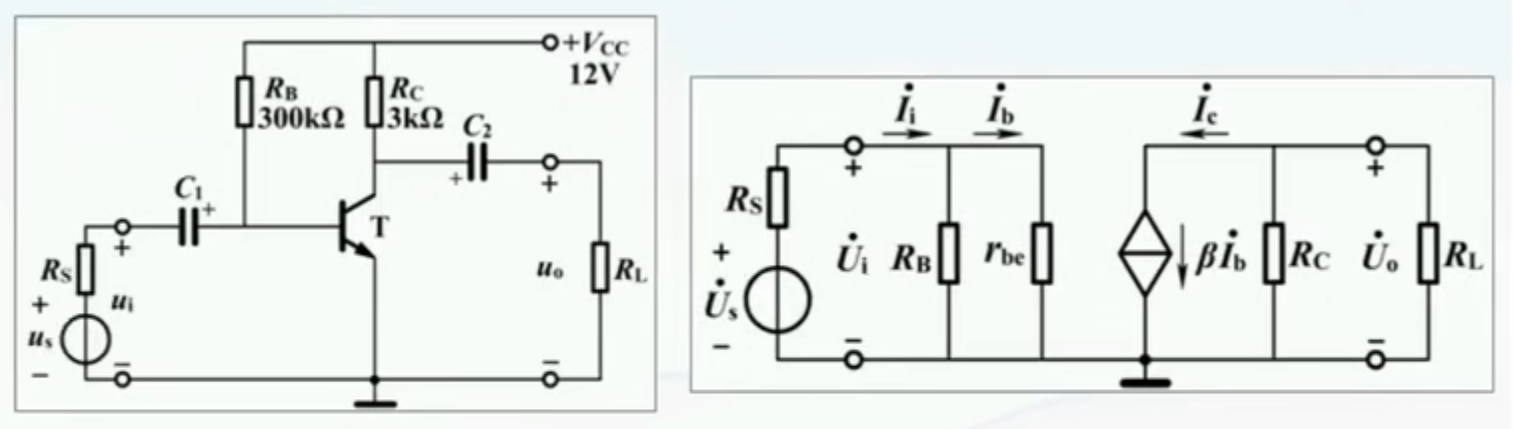
\includegraphics[scale=0.4]{image/image1}
\end{figure}
\begin{align*}
I_{BQ} &= \frac{V_{CC} - U_{BEQ}}{R_B} \approx \frac{V_{CC}}{R_B} = \frac{12}{300} = 0.04mA \\
I_{EQ} &\approx I_{CQ} = \beta I_{BQ} = 50 \times 0.04 = 2mA \\
r_{be} &= 100 + (1 + \beta)\frac{26mV}{I_E mA} \\
       &= 100 + (1+ 50) \times \frac{26}{2} \\
       &\approx 760\Omega = 0.76\Omega \\
R^{'}_L &= R_C \parallel R_L = \frac{3 \times 2}{3 + 2} = 1.2k\Omega
\end{align*}
\flushleft{1.空载电压放大倍数:$\dot{A}_u = -\beta\frac{R_C}{r_{be}} = -50\times\frac{3}{0.76} = -197.4$}
\flushleft{2.负载电压放大倍数:$\dot{A}_u = -\beta\frac{R_C \parallel R_L}{r_{be}} = -50\times\frac{1.2}{0.76} = -78.9$}
\flushleft{3.输入电阻:$R_i = R_B \parallel r_{be} \approx r_{be} = 0.76k\Omega$}
\flushleft{4.输出电阻:$R_o = R_C = 3k\Omega$}
\flushleft{5.源电压放大倍数:$\dot{A}_{us} = -\beta\frac{R^{'}_L}{R_S + r_{be}} = -50\times\frac{1.2}{0.5 + 0.76} = -47.6$}

\section{静态工作点的稳定}
\flushleft{由直流通路和KCL得:$I_1 = I_2 + I_B$}
\flushleft{设:$I_1 \approx I_2 >> I_B$}
\flushleft{则:$I_1 \approx I_2 \approx \frac{U_{CC}}{R_{B1} + R_{B2}} \newline V_B = I_2R_{B2} \approx \frac{R_{B2}}{R_{B1} + R_{B2}}U_{CC}$}
\flushleft{可认为$V_{B}$的大小与晶体管参数无关、不受温度影响,仅为$R_{B1}$和$R_{B2}$的分压电路所固定。}
\flushleft{在电路中引入发射极电阻后,可得:$U_{BE} = V_B - V_E = V_B - I_E R_E$}
\flushleft{稳定静态工作点的物理流程:}
\begin{gather*}
T\uparrow \rightarrow I_C\uparrow \rightarrow V_E\uparrow \rightarrow U_{BE}\downarrow \rightarrow I_B\downarrow \rightarrow I_C\downarrow
\end{gather*}

\section{分压式偏置放大电路的静态分析}
\begin{gather*}
V_B = \frac{R_{B2}}{R_{B1} + R_{B2}}V_{CC} \\
I_{CQ} \approx I_{EQ} = \frac{V_B - U_{BEQ}}{R_E} \approx \frac{V_B}{R_E} \\
I_{BQ} = \frac{I_{CQ}}{\beta} \\
U_{CEQ} = V_{CC} - I_{CQ}(R_C + R_E)
\end{gather*}
\flushleft{在电流分流时忽略$I_{BQ}$的大小,但是依旧需要通过$I_{CQ}$计算出$I_{BQ}$的值。}

\newpage

\section{分压式偏置放大电路的动态分析}
\begin{align*}
\dot{U}_i &= \dot{I}_b r_{be} + \dot{I}_e R_E \\
          &= \dot{I}_b r_{be} + (1 + \beta)\dot{I}_b R_E \\
          &= \dot{I}_b [r_{be} + (1 + \beta) R_E]
\end{align*}
\begin{gather*}
\dot{U}_o = -\dot{I}_c R^{'}_L = -\beta \dot{I}_b R^{'}_L \\
\dot{A}_{u} = \frac{\dot{U}_o}{\dot{U}_i} = -\frac{\beta\dot{I}_b R^{'}_L}{\dot{I}_b[r_{be} + (1 + \beta)R_E]} = -\beta\frac{R^{'}_L}{r_{be} + (1 + \beta)R_E]} \\
R_i = R_{B1} \parallel R_{B2} \parallel [r_{be} + (1 + \beta)R_E] \\
R_o = R_C
\end{gather*}

\end{document}
